
\documentclass[]{emulateapj}
\usepackage{amsmath}
\begin{document}
\author{Draft}


\section{Gravitational Lens model}

\subsection{interpretation}
- C06 suggest the presence of an interacting dusty galaxy in their HST
observations, which BJB+08 calls it the F component. The lensed images of the
ABCDE 
components coincide with our CO data (see mom0 on HST and channel map),
evidently CO emission coming from the AGN host galaxy. 
- one of the red channels in our lens model suggests a second source component,
which is consistent with the spatially offset dusty source (see mom0 on HST,
which 
the red velocity component coincides with this F component)

%%%%%%%%%%%%%%%%%%%%%%%%
+ Compare our lens model parameters on the mass distribution of the lensing
galaxy with literature (specifically SIE model in C06)
	- C06: SIE model shows position of lensing mass is offset by (-0.015",
-0.041" from obs. (i.e. light centroid)); PA = -73.6, ellipticity = 0.45,
theta_R = 1.84" +/- 0.01 
	- Our model lens parameters (median):
		- file: WRITEUP/MedianLensModelParams.txt
		- lensing gal. position is consistent with C06, 
		- Einstein radius: consistent with C06
		- PA: consistent within errors
		- Axial ratio: consistent within errors
%%%%%%%%%%%%%%%%%%%%%%%%%


\begin{figure}[tbph]
\centering
\includegraphics[width=0.50\textwidth]{../Figures/Pseudointegrated_datamodel.ep
s}
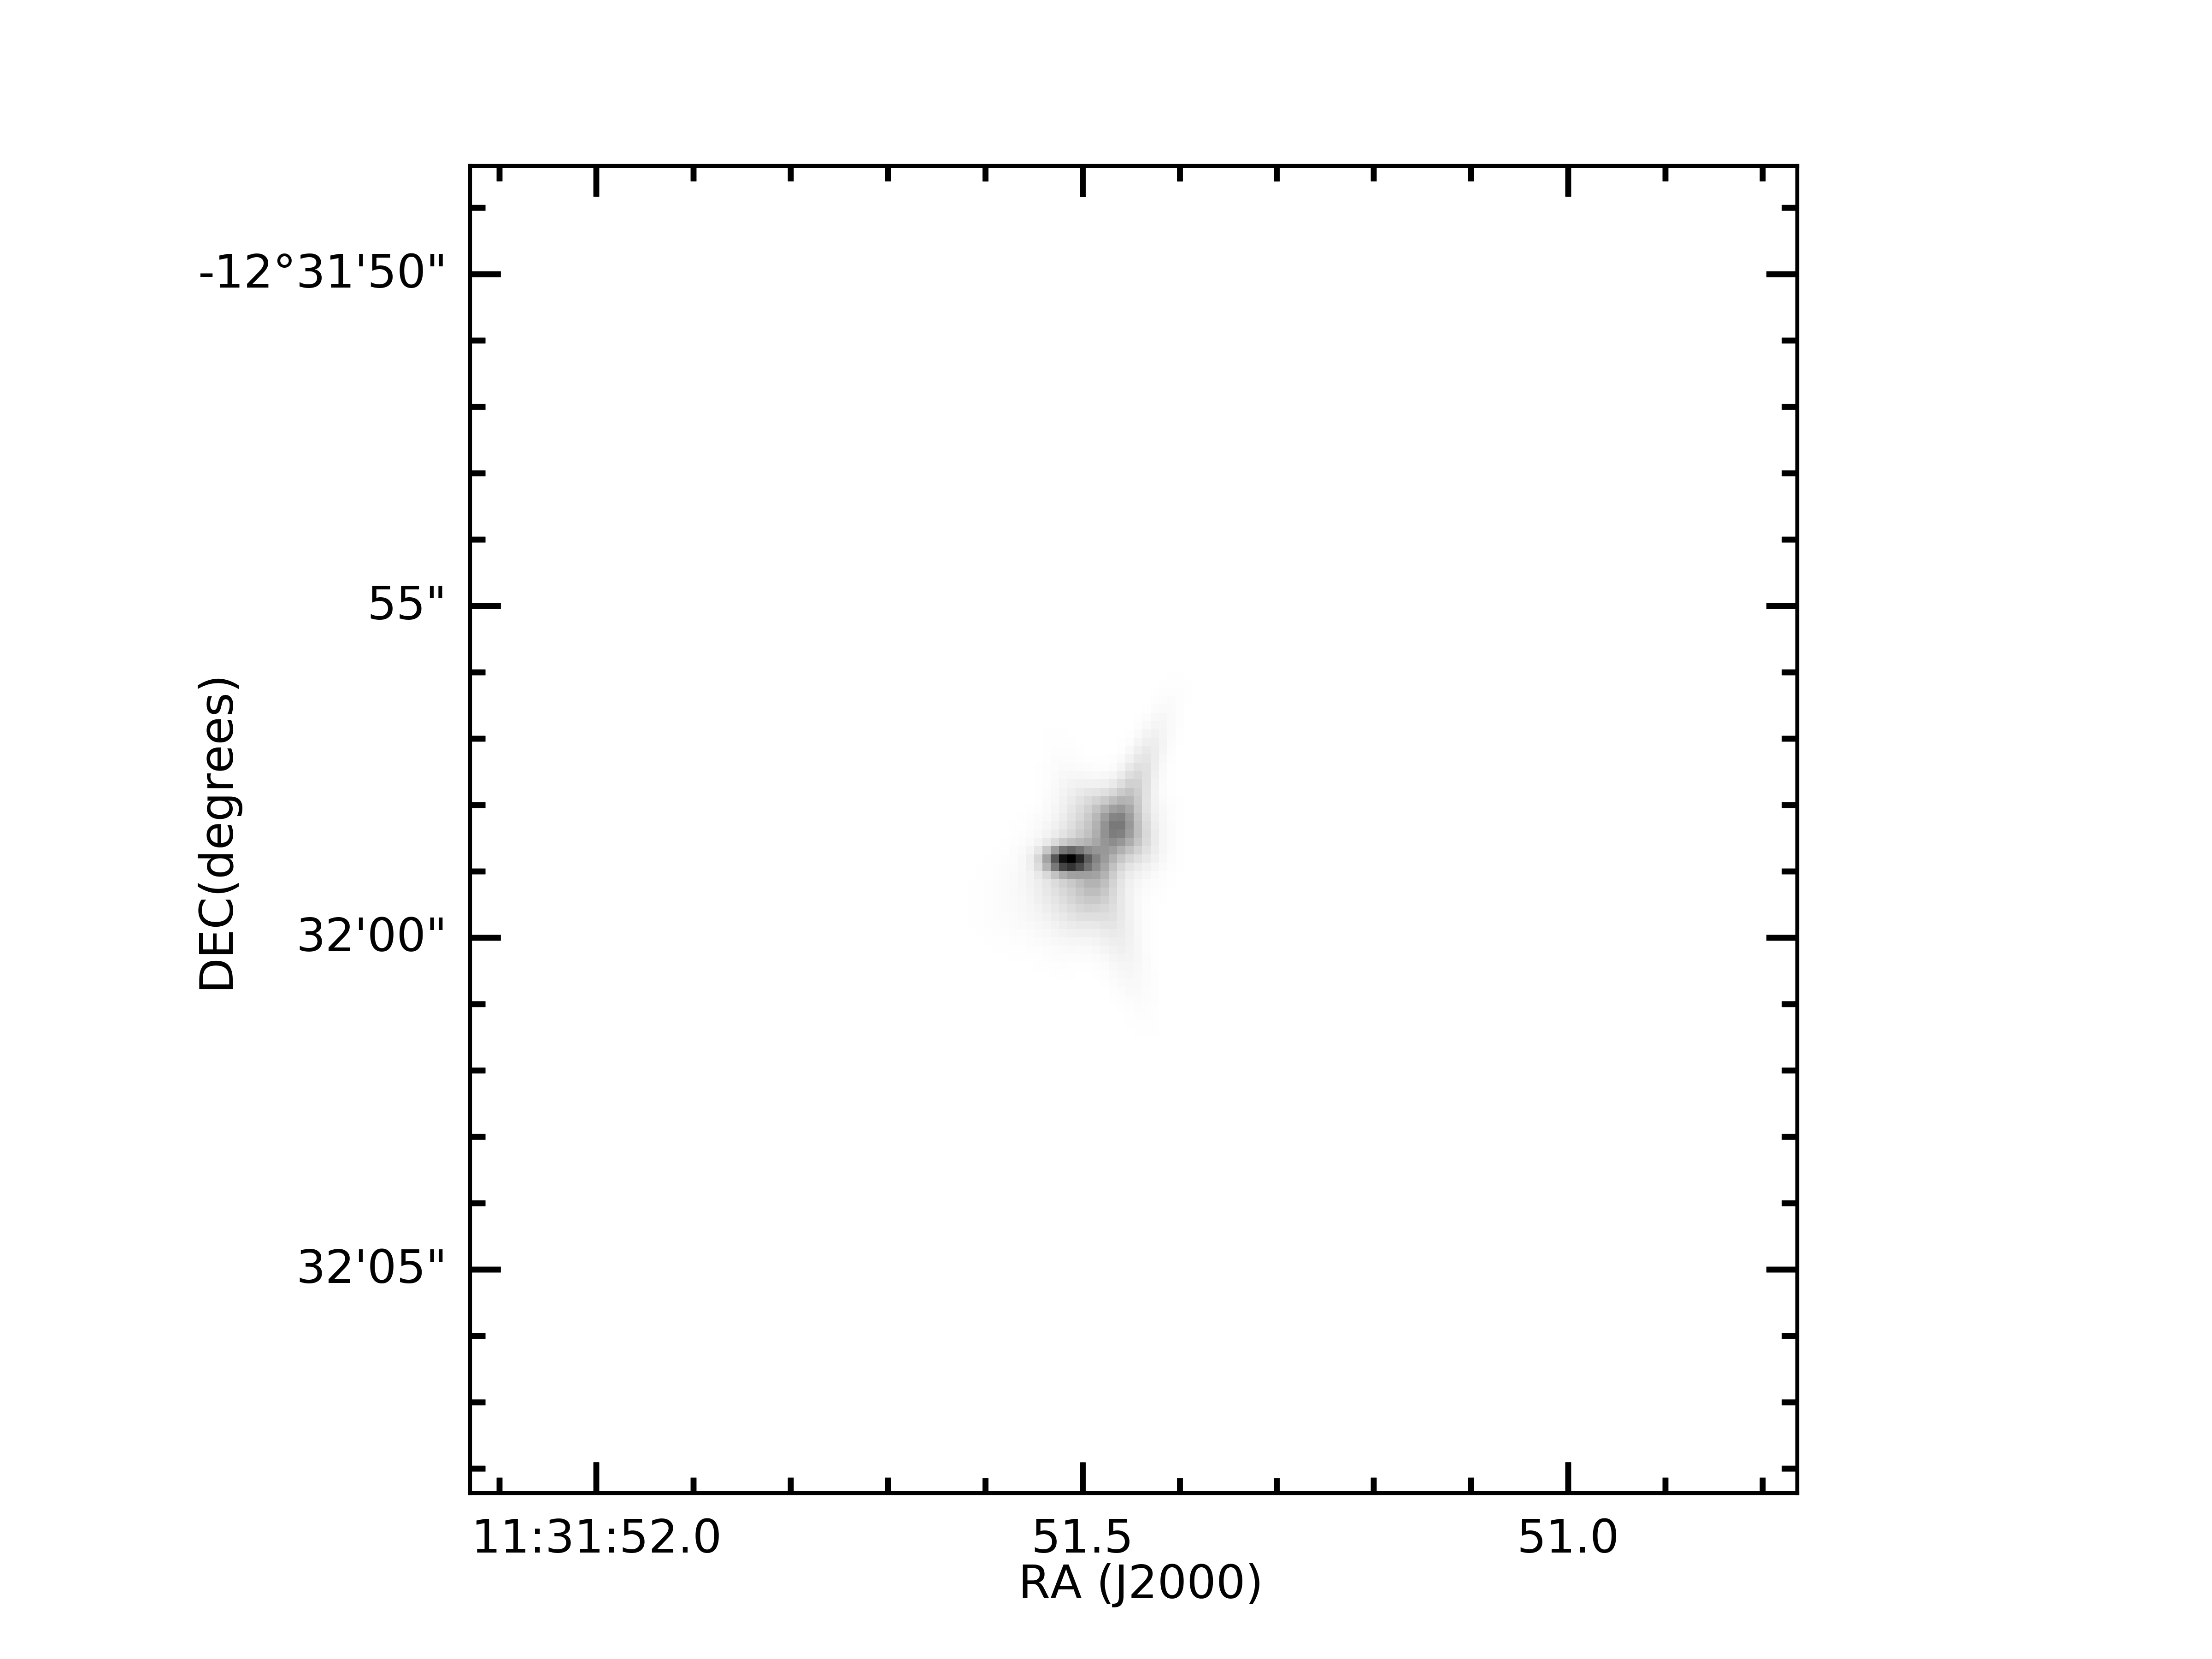
\includegraphics[width=0.50\textwidth]{../Figures/SourcesPlane.png}
\caption{
Pseudo observed 0th moment map in the lens plane. (left)
Pseudo 0th moment map in the source plane. (right)
\label{fig:}}
\end{figure}


%\begin{figure*}[tbph]
%\centering
%\caption{
%\label{fig:}}
%\end{figure*}


\begin{figure*}[tbph]
\centering
\includegraphics[width=0.80\textwidth]{../Figures/PseudoRGB_Lensed_SB_double.ep
s}
\caption{
velocity gradient of the lens model in the lens plane (left), source plane
(right).
\label{fig:}}
\end{figure*}


%\begin{figure*}[tbph]
%\centering
%\includegraphics[width=0.8\textwidth]{}
%\includegraphics[width=0.65\textwidth]{}
%\caption{
%\label{fig:}}
%\end{figure*}

\end{document}